\chapter{Experimental Analysis}
\label{chap:analysis}

\section{Pipeline Results}
\label{sec:p3-results}

\subsection{Unsupervised Anomaly Detection with PatchCore (P3)}

\subsubsection{Evaluation protocol}

All results are obtained through a database-driven evaluation that, for each
normal reference frame, (i) builds the memory bank from augmented variants of the
reference (excluding the original), (ii) calibrates the threshold on independent
variants, (iii) scores the original reference as the normal test sample, and
(iv) scores the obstructed frames linked to that reference. Scores are
normalised per camera as $(s - \mu_i)/\sigma_i$ before aggregating the AUROC,
while threshold-based metrics (false-positive rate FPR, true-positive rate TPR,
and $F_1$) use the per-camera threshold $\theta_i$ so that each binary decision
reflects its own calibration.

The evaluation is organised in two macro-phases (Table~\ref{tab:p3-phases}),
reflecting the two roles of the datasets introduced in
Chapter~\ref{chap:method}. \textbf{Phase~1} runs on the synthetic copy-paste
corpus (D1, split \emph{test}, doors and corridors together; about $990$ reference
frames, each with one or more obstructed variants). Because a copy-paste
obstruction leaves the background unchanged, only the pasted object is anomalous
and the discrimination problem is near-saturated (AUROC $\approx 1$); Phase~1 is
therefore not a measure of headline accuracy but a \emph{calibration study} - how
to build the memory bank, place the decision threshold, and add shadow and light
augmentation so that a single operating point stays robust to non-obstacle
disturbances. Its internal structure is a progressive ablation, each component
introduced in response to a failure mode identified empirically. \textbf{Phase~2}
runs on the real on-site test set (D2): it measures operational accuracy on real
doors with manually annotated gating, and here the reported metrics - recall,
precision, $F_1$, accuracy - are the ones that matter.

\begin{table}[h]
  \centering
  \begin{tabular}{c l p{4.3cm} p{3.2cm}}
    \hline
    Phase & Dataset & Focus & Key metrics \\
    \hline
    1 & D1 (synthetic copy-paste) & Calibration: memory bank, decision threshold, shadow/light augmentation & FPR, threshold stability \\
    2 & D2 (real, on-site) & Real-world accuracy with manual polygon gating & Recall, precision, $F_1$, accuracy \\
    \hline
  \end{tabular}
  \caption{The two macro-phases of the P3 evaluation.}
  \label{tab:p3-phases}
\end{table}

\subsubsection{Phase 1: calibration on the synthetic corpus (D1)}

On D1 the discriminative problem is essentially solved before any tuning, so the
goal of this phase is to convert the latent separability into a single, robust
operating point. The ablation introduces one component at a time, each in
response to a failure mode observed in the previous step.

\paragraph{Baseline.}
The baseline ($n_{\mathrm{aug}}=15$, $n_{\mathrm{cal}}=10$, no disturbance
augmentation, $k=3$) cleanly separates normal from obstructed scenes
(Table~\ref{tab:p3-phaseA}). The near-perfect AUROC and the gap of several
standard deviations between the class means confirm that obstacle patches fall
well outside the distribution of normal door and corridor patches. The residual
$0.5\%$ FPR corresponds to about five false alarms over $990$ frames.
Discrimination is thus not the bottleneck; what remains is to keep this operating
point stable once realistic disturbances enter the scene.

\begin{table}[h]
  \centering
  \begin{tabular}{lccc}
    \hline
    Category & Mean score & Std & Rate \\
    \hline
    Normal & $2.309$ & $0.156$ & FPR $0.5\%$ \\
    Obstructed & $4.648$ & $0.348$ & TPR $100\%$ \\
    AUROC & \multicolumn{3}{c}{$\approx 1.000$} \\
    \hline
  \end{tabular}
  \caption{Phase 1 baseline on the synthetic test set.}
  \label{tab:p3-phaseA}
\end{table}

\paragraph{Shadow vulnerability.}
A test set of shadow-augmented normal scenes (one synthetic variant per
reference, $k_s\in[1,3]$ stacked shadows) is scored against the baseline model.
These are normal scenes with no obstruction, yet $90.1\%$ are flagged as anomalous
(Table~\ref{tab:p3-phaseB}). Shadow patches - dark, smoothly-bordered regions -
are out of distribution for a bank built from shadow-free photometric variants, so
they receive high anomaly scores, high enough to exceed a threshold calibrated on
clean scenes.

\begin{table}[h]
  \centering
  \begin{tabular}{lcccc}
    \hline
    Category & Mean & Std & Range & Rate \\
    \hline
    Normal & $2.309$ & $0.156$ & $[1.87, 3.13]$ & FPR $0.5\%$ \\
    Shadow normal & $3.189$ & $0.495$ & $[2.10, 4.51]$ & FPR $90.1\%$ \\
    Obstructed & $4.648$ & $0.348$ & $[3.54, 5.87]$ & TPR $100\%$ \\
    \hline
  \end{tabular}
  \caption{Phase 1, shadow vulnerability: shadow-normal scores overlap the
  obstructed range $[3.54, 4.51]$.}
  \label{tab:p3-phaseB}
\end{table}

The shadow scores (mean $3.19$) land above the clean normals (mean $2.31$) but
still below the obstructions (mean $4.65$): a shadow is more anomalous than a clean
scene, yet clearly less than a real obstruction. The $90\%$ FPR therefore comes
from the decision threshold - calibrated on clean variants alone, it sits at
$\approx 2.47$, below the entire shadow band - and not from any inability to tell
shadows from obstructions, a distinction made precise later
(Section ``Discrimination versus calibration'').

\paragraph{Shadow augmentation and calibration stabilisation.}
Introducing shadow augmentation in the build phase, then decoupling and pooling
the calibration, traces a clear path (Table~\ref{tab:p3-phaseC}). Coupling the
build and calibration probabilities ($p_{\mathrm{sh}} =
p_{\mathrm{sh}}^{\mathrm{cal}} = 0.4$) reduces shadow FPR by two orders of
magnitude but over-inflates the threshold, dropping TPR to $70.6\%$; the cause is- [ ] Aggiungere al dataset copy-paste varianti con oggetti tagliati a metà dalla
      scena.
a long tail in the per-camera threshold distribution, where $12\%$ of cameras
generate $86\%$ of all false negatives. Decoupling
($p_{\mathrm{sh}}^{\mathrm{cal}} = 0.1$, $n_{\mathrm{cal}} = 30$) recovers TPR but
swings to an over-permissive operating point. Replacing the per-camera $\sigma_i$
with the pooled median $\sigma_{\mathrm{pop}} = 0.300$ at $k=4$ eliminates the
residual threshold variance and reaches the best operating point.

\begin{table}[h]
  \centering
  \begin{tabular}{lccccc}
    \hline
    Configuration & Clean FPR & Shadow FPR & TPR & $F_1$ & $\sigma_\theta$ \\
    \hline
    Baseline (no aug) & $0.5\%$ & $90.1\%$ & $100\%$ & $0.688$ & $0.158$ \\
    Coupled ($k=3$) & $0.0\%$ & $2.1\%$ & $70.6\%$ & $0.818$ & $0.539$ \\
    Decoupled ($k=3$) & $0.0\%$ & $28.4\%$ & $99.4\%$ & $0.873$ & $0.388$ \\
    Decoupled ($k=4$) & $0.0\%$ & $13.5\%$ & $93.4\%$ & $0.903$ & $0.497$ \\
    \textbf{Pooled $\sigma$ ($k=4$)} & $\mathbf{0.0\%}$ & $\mathbf{12.2\%}$ & $\mathbf{99.8\%}$ & $\mathbf{0.941}$ & $\mathbf{0.137}$ \\
    \hline
  \end{tabular}
  \caption{Phase 1, shadow augmentation and calibration stabilisation.
  $\sigma_\theta$ is the standard deviation of the per-camera thresholds.}
  \label{tab:p3-phaseC}
\end{table}

Pooling collapses the threshold range from $[2.28, 6.09]$ to $[3.24, 4.16]$ (a
$73\%$ reduction in $\sigma_\theta$) and removes the pathological tail entirely:
no camera exceeds $\theta = 4.16$ and TPR stays at $99.3\%$ or higher in every
threshold bucket. The $3.8$ percentage-point $F_1$ gain is due entirely to
variance reduction, not to any change in the backbone, whose AUROC stays at
$0.998$. The choice $k=4$ follows a conservative four-sigma rule and was not
tuned on the test set: the $F_1$-optimal value is about $3.9$, but reporting it
would constitute test-set tuning.

\paragraph{Light augmentation ablation.}
The symmetric counterpart of the shadow failure mode - localised brightness
excess - is evaluated on a light-augmented test set ($\approx 1100$ normal
scenes) at $k=4$, pooled $\sigma$, $n_{\mathrm{cal}}=30$.
Five configurations are compared (Table~\ref{tab:p3-phaseE}), where the
\emph{budget} $p_{\mathrm{sh}} + p_{\mathrm{li}}$ is the expected disturbance
probability per variant, a proxy for total augmentation intensity. A fifth
fair-budget control (L4) disentangles two effects that L2/L3 confound: increased
coverage (adding the light type) and increased total intensity.

\begin{table}[h]
  \centering
  \begin{tabular}{lcccccc}
    \hline
    Config & $p_{\mathrm{sh}}$ & $p_{\mathrm{li}}$ & Budget & Shadow FPR & Light FPR & $F_1$ \\
    \hline
    L0 shadow-only & $0.4$ & $0.0$ & $0.40$ & $12.2\%$ & $5.8\%$ & $0.917$ \\
    L1 light-only & $0.0$ & $0.4$ & $0.40$ & $37.7\%$ & $23.2\%$ & $0.767$ \\
    \textbf{L2 SL-15} & $0.4$ & $0.4$ & $0.80$ & $\mathbf{2.2\%}$ & $\mathbf{0.30\%}$ & $\mathbf{0.982}$ \\
    L3 SL-25 & $0.4$ & $0.4$ & $0.80$ & $1.1\%$ & $0.10\%$ & $0.982$ \\
    L4 fair-budget & $0.23$ & $0.23$ & $0.46$ & $11.2\%$ & $4.6\%$ & $0.929$ \\
    \hline
  \end{tabular}
  \caption{Phase 1 light-augmentation ablation. TPR is $\geq 97.7\%$ throughout.
  L0/L2 use $n_{\mathrm{aug}}=15$, L3 uses $n_{\mathrm{aug}}=25$.}
  \label{tab:p3-phaseE}
\end{table}

Four findings emerge. First, \emph{light is a milder disturbance than shadow}:
even with no light coverage (L0) the light FPR is $5.8\%$, below the $12.2\%$
shadow FPR, because a light beam pushes features less out of distribution than a
cast shadow. Second, \emph{adding light augmentation works and helps shadows
too}: from L0 to L2 the light FPR falls about nineteen-fold while the shadow FPR
also improves rather than degrading. Third, L1 confirms that shadow augmentation
is \emph{structural, not incidental}: removing it collapses the per-camera
threshold and inflates all FPRs, light included - light augmentation is a
complement to shadow augmentation, not a substitute. Fourth, the fair-budget
control shows that \emph{the headline gain is mostly a budget effect}: L2/L3 apply
twice the augmentation of L0, and the mean threshold grows monotonically with
budget, tracking the FP reduction; at equal budget (L4 vs.\ L0) diversification
alone yields only a small, cost-free improvement. The recommended configuration
is SL-15 ($F_1 = 0.982$, light FPR $0.30\%$, shadow FPR $2.2\%$, recall $99.0\%$);
SL-25 halves the FPRs again but trades recall for identical $F_1$ at a markedly
longer build time, justified only when minimal FP is required. As established in
Chapter~\ref{chap:setup}, light and shadow FPR are not directly comparable; only
within-category readings are valid.

\paragraph{Discrimination versus calibration.}
A cross-cutting question determines what the pipeline can legitimately claim: do
the interventions improve the model's \emph{discriminative capacity} or only the
\emph{placement of the threshold}? The clean metric is the per-camera AUROC -
the probability that an obstruction scores higher than a normal variant of the
\emph{same} camera, on raw scores, averaged over cameras. Within a camera $\mu_i$
and $\sigma_i$ are constant, so raw and normalised scores differ by an affine
transform that preserves ranking; the per-camera AUROC is therefore invariant to
both threshold and normalisation and isolates intrinsic discrimination.

\begin{table}[h]
  \centering
  \begin{tabular}{lccccc}
    \hline
    Config & raw AUROC & per-cam AUROC (shadow) & shadow FPR & TPR & $F_1$ \\
    \hline
    no-aug & $0.9969$ & $0.996$ & $90.1\%$ & $100\%$ & $0.688$ \\
    shadow04 & $0.9981$ & $0.996$ & $2.1\%$ & $70.6\%$ & $0.818$ \\
    decoupled & $0.9981$ & $0.996$ & $28.4\%$ & $99.4\%$ & $0.873$ \\
    decoupled $k=4$ & $0.9981$ & $0.996$ & $13.5\%$ & $93.4\%$ & $0.903$ \\
    pooled & $0.9981$ & $0.996$ & $12.2\%$ & $99.8\%$ & $0.941$ \\
    \hline
  \end{tabular}
  \caption{Controlled comparison: shadow FPR swings $40\times$ while raw and
  per-camera AUROC stay fixed.}
  \label{tab:p3-disc}
\end{table}

The per-camera AUROC is saturated and nearly invariant to augmentation
(Table~\ref{tab:p3-disc}): clean separation is perfect everywhere, the shadow
value stays at $0.996$ across the whole path - even with no shadow augmentation -
and the light value is likewise saturated ($0.997$ to $1.000$). The shadow FPR
meanwhile swings
from $2.1\%$ to $90\%$ to $12\%$ while the raw AUROC is fixed at $0.9981$. The
mechanism is a \emph{threshold shift, not a re-ordering}: the score distributions
themselves barely move (shadowed-normal mean $3.19 \to 3.14$, obstructed
$4.65 \to 4.66$), so within each scene an obstruction still outscores a shadow
exactly as before and the per-camera AUROC is unchanged. What moves is the
decision threshold $\theta_i = \mu_i + k\sigma$: calibrated on clean variants
alone it sits low (mean $\approx 2.47$), \emph{below} the shadow band, so $90\%$ of
shadows exceed it; once disturbance variants enter the calibration set (raising
$\mu$ and $\sigma$) and $\sigma$ is pooled, $\theta$ rises (mean $\approx 3.74$)
\emph{above} the shadow band but still below the obstructions, cutting the shadow
FPR to $\approx 12\%$ (Figure~\ref{fig:p3-calib}). None of this adds discriminative
power - it places a single threshold so that the already-excellent latent
discrimination becomes usable.

\begin{figure}[h]
  \centering
  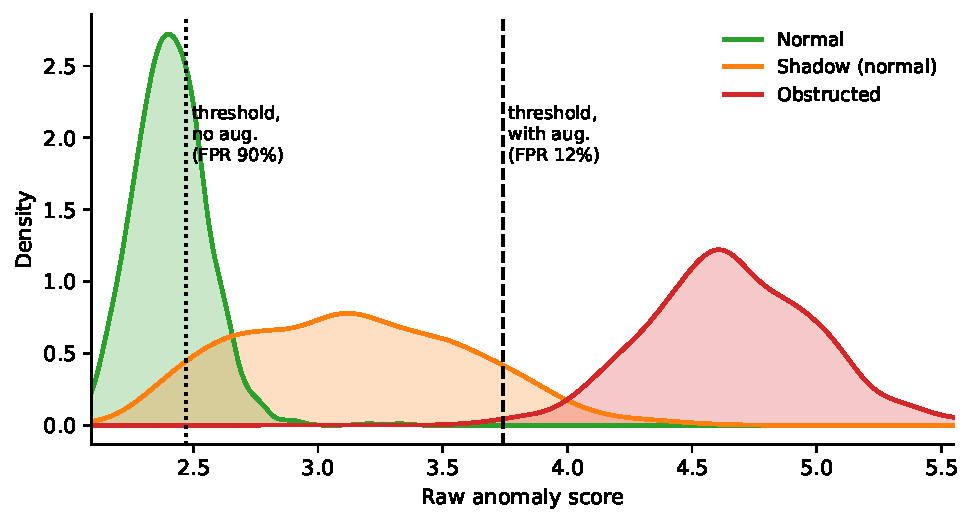
\includegraphics[width=0.85\textwidth]{images/patchCore/p3_calibration_shift.pdf}
  \caption{Calibration, not discrimination. The raw score distributions of normal,
  shadowed-normal, and obstructed scenes are essentially unchanged by augmentation,
  so their overlap - and the per-camera ranking (AUROC $0.996$) - is fixed. Only
  the decision threshold moves: calibrated on clean variants it sits at
  $\approx 2.47$ (dotted), inside the shadow band, flagging $90\%$ of shadows; with
  disturbance-augmented, pooled calibration it rises to $\approx 3.74$ (dashed),
  above the shadow band but still below the obstructions, cutting the shadow FPR to
  $\approx 12\%$. The thresholds shown are means of the per-camera values.}
  \label{fig:p3-calib}
\end{figure}

This conclusion holds on a test set where discrimination is near-saturated by
design (copy-paste obstructions on the same background: only the object is
anomalous, a strong signal, AUROC $\approx 1$). On harder data - real
obstructions, variable backgrounds - the absolute AUROC values could differ; the
per-camera AUROC argument is a claim about this dataset's regime and is stated as
such.

\subsubsection{Phase 2: real-world accuracy with manual gating (D2)}

Phase~2 is the first evaluation on real photographs rather than copy-paste
composites, and the first to report operational accuracy. The test set is D2: six
real doors photographed on site (a mix of opaque and glass doors), each with one
manually annotated reference frame, comprising $30$ real obstructed images, $30$
unobstructed images, and the six references. Consistent with the fixed-camera
assumption, all shots of a door share the same framing, so the negatives measure
the FPR under normal content and illumination variability at fixed geometry. The
full pipeline is active: pooled $\sigma$ plus connected-component gating
($\tau = 10$) against the hand-annotated door-frame polygons
(the gating rule is illustrated stage by stage in
Figure~\ref{fig:p3-gating}).

Validated on the synthetic suites, $k=4$ proved too conservative on real scenes;
lowering it to $k=3$ raises recall at no FPR cost
(Table~\ref{tab:p3-phaseD}; Figure~\ref{fig:p3-d2-metrics}). Because the pooled $\operatorname{median}(\sigma) =
0.213$ is a shared constant, lowering $k$ shifts every threshold down by the same
amount without widening the distribution - the per-camera variance amplification
of the naive rule does not reappear.

\begin{table}[h]
  \centering
  \begin{tabular}{lccc}
    \hline
    Metric & $k=4$ & $k=3$ & $\Delta$ \\
    \hline
    Recall (TPR) & $83.3\%$ & $\mathbf{90.0\%}$ & $+6.7$ pp \\
    FPR & $3.3\%$ & $3.3\%$ & invariant \\
    Precision & $96.2\%$ & $96.4\%$ & $+0.2$ pp \\
    $F_1$ & $0.893$ & $\mathbf{0.931}$ & $+0.038$ \\
    Accuracy & $90.0\%$ & $93.3\%$ & $+3.3$ pp \\
    \hline
  \end{tabular}
  \caption{Phase 2: recalibration of $k$ on the real test set.}
  \label{tab:p3-phaseD}
\end{table}

\begin{figure}[h]
  \centering
  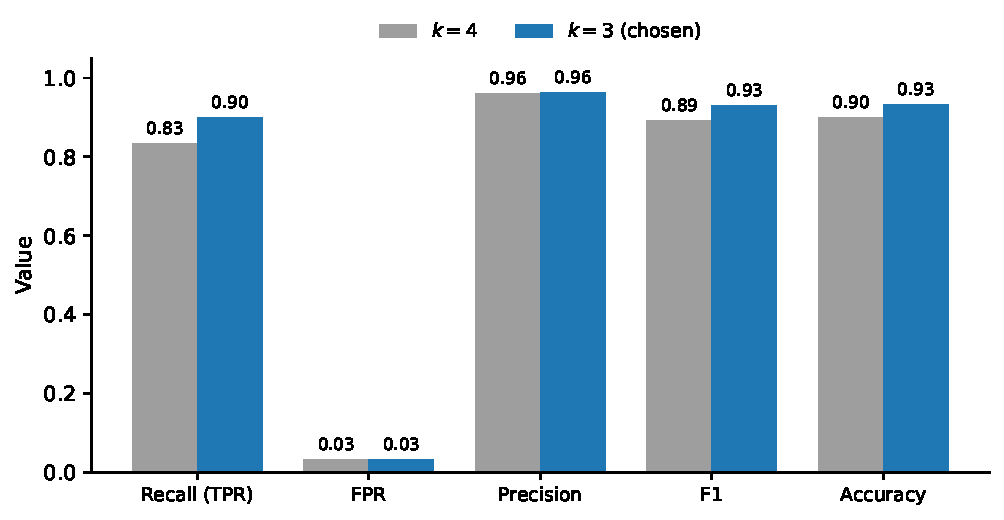
\includegraphics[width=0.8\textwidth]{images/patchCore/p3_d2_metrics.pdf}
  \caption{Operating-point metrics on the real test set (D2), at the
  synthetic-validated $k=4$ and the recalibrated $k=3$. Lowering $k$ raises recall
  ($83.3\% \to 90.0\%$), $F_1$ ($0.893 \to 0.931$) and accuracy
  ($90.0\% \to 93.3\%$) at unchanged FPR ($3.3\%$) and precision.}
  \label{fig:p3-d2-metrics}
\end{figure}

Comparing the two runs separates the false negatives by cause
(Figure~\ref{fig:p3-d2-scores}). Two are
\emph{calibration-limited} and are recovered at $k=3$ through the two distinct
stages where $k$ acts: one is a decision-stage miss (a valid gated component
scored just below the decision threshold at $k=4$), the other a
binarisation-stage miss (the obstruction's anomaly peak fell just below the local
binarisation threshold at $k=4$, leaving an empty binary map). The latter shows
that $\theta$ controls not only the decision but which pixels exist for gating to
evaluate, so an overly high $k$ can erase a low-contrast obstruction before
gating sees it. Three remain zeroed even at $k=3$ and are \emph{gating-limited}:
the prototypical case is a free-standing floor fan whose wide head sits on the
door panel (excluded from the frame mask by design) while its thin pole is the
only part touching the frame and threshold (Figure~\ref{fig:p3-d2-fn-fan}). The
pole is too slender to register as anomalous: only the head produces a strong
response, so the fan does not form a single connected anomaly component that
bridges the panel to a frame region. The head's component lies entirely in the
excluded panel area and has no anomalous link reaching the frame, so gating zeros
it. PatchCore detects the obstruction correctly; the failure is purely geometric,
confirming the structural limitation anticipated in Chapter~\ref{chap:method}:
the grounded-obstacle assumption holds for wide-profile objects (carts,
wheelchairs, bins) but not for thin-stemmed ones (fans, coat racks, sign posts).
A single FP is a glass door whose background changed behind the panel
(Figure~\ref{fig:p3-d2-fp-blind}): with the external rolling shutter lowered, the
view through the glass differs entirely from the reference frame, so the whole
panel area lights up in the anomaly map and the pooled threshold is exceeded -
a calibration limit of the fixed-background assumption rather than a gating
failure. With
order-of-tens samples, these numbers are a qualitative validation of the complete
pipeline, not a production benchmark.

\begin{figure}[h]
  \centering
  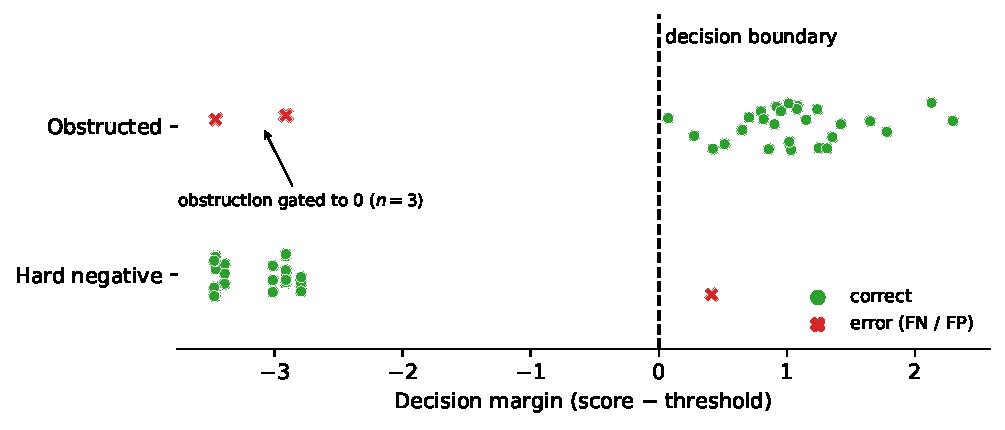
\includegraphics[width=0.85\textwidth]{images/patchCore/p3_d2_scores.pdf}
  \caption{Per-sample decision margin (score $-$ per-camera threshold) on D2 at
  $k=3$; the decision boundary is the line at $0$. The $30$ obstructed and $30$
  hard-negative frames are cleanly separated except for three obstructions gated to
  a zero score - the gating-limited false negatives, including the thin-stemmed
  floor fan - and one hard-negative false positive (a glass door whose background
  changed behind the panel).}
  \label{fig:p3-d2-scores}
\end{figure}

\begin{figure}[h]
  \centering
  \begin{subfigure}{0.42\textwidth}
    \centering
    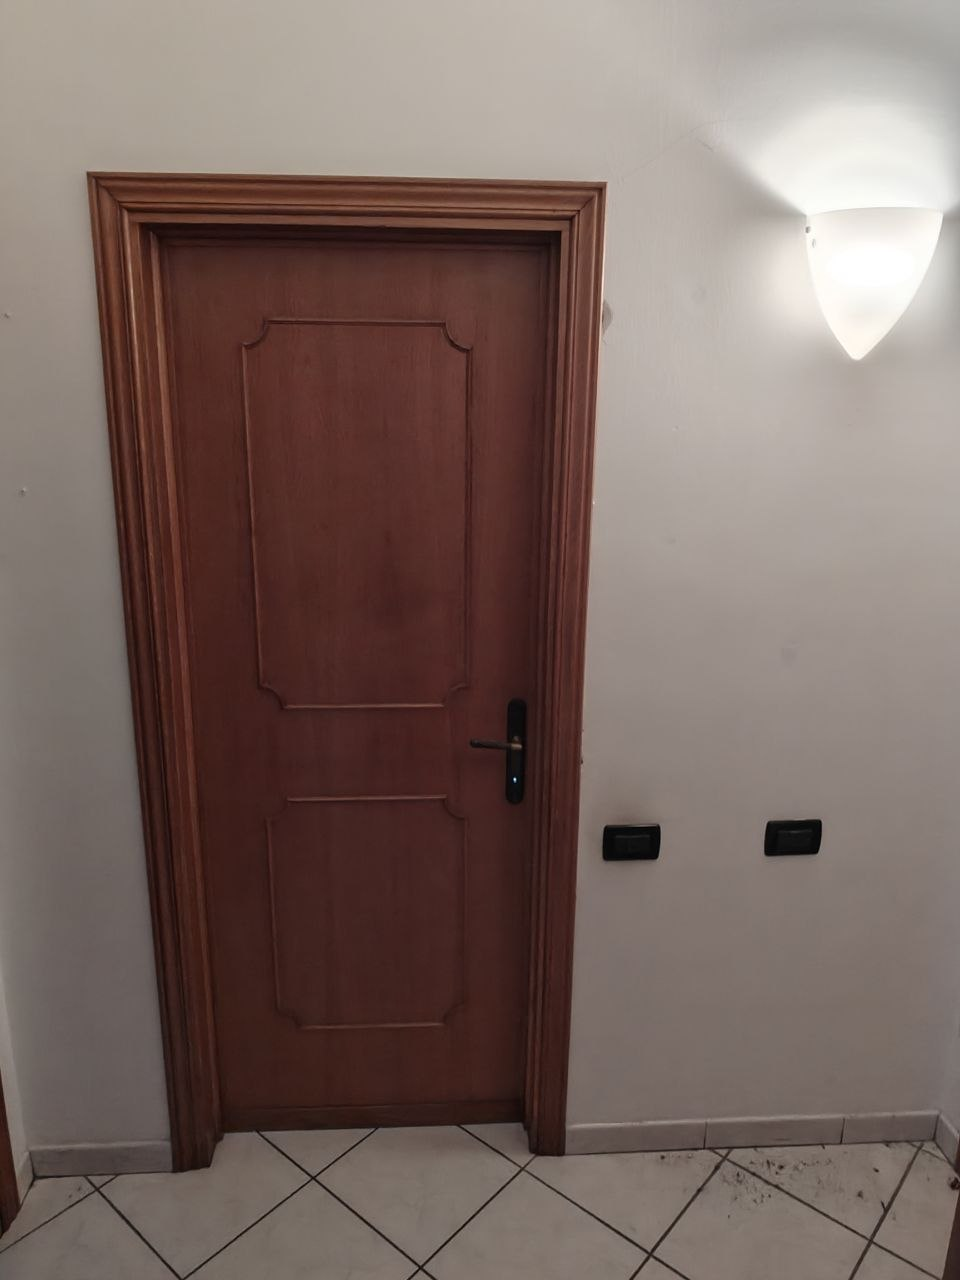
\includegraphics[width=\textwidth]{images/patchCore/p3_d2_fn_fan_ref.jpg}
    \caption{Reference (normal)}
    \label{fig:p3-d2-fn-fan-ref}
  \end{subfigure}
  \hfill
  \begin{subfigure}{0.42\textwidth}
    \centering
    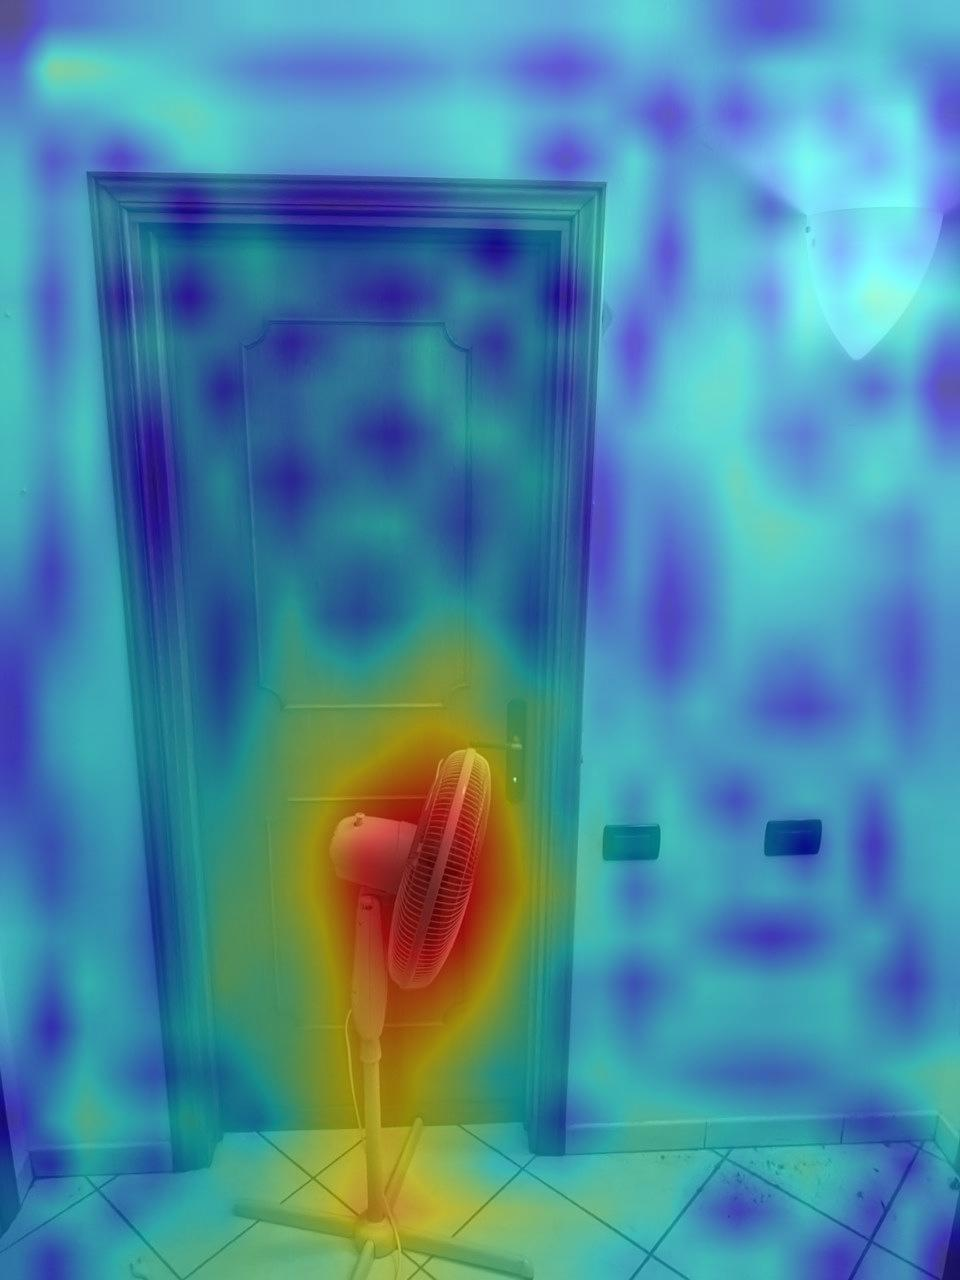
\includegraphics[width=\textwidth]{images/patchCore/p3_d2_fn_fan_heatmap.jpg}
    \caption{Anomaly heatmap}
    \label{fig:p3-d2-fn-fan-heatmap}
  \end{subfigure}
  \caption{Gating-limited false negative (worst case, score $0.000$). PatchCore
  correctly flags the fan head and base as anomalous in the heatmap, but the head
  rests on the door panel, which is excluded from the frame mask by design. The
  thin pole - the only part touching the frame and threshold - is too slender to
  register as anomalous, so the fan does not form a single connected anomaly
  component bridging the panel to a frame region. The head's component lies
  entirely in the excluded panel area with no anomalous link reaching the frame,
  and gating therefore zeros it. The failure is purely geometric, not a detection
  error.}
  \label{fig:p3-d2-fn-fan}
\end{figure}

\begin{figure}[h]
  \centering
  \begin{subfigure}{0.42\textwidth}
    \centering
    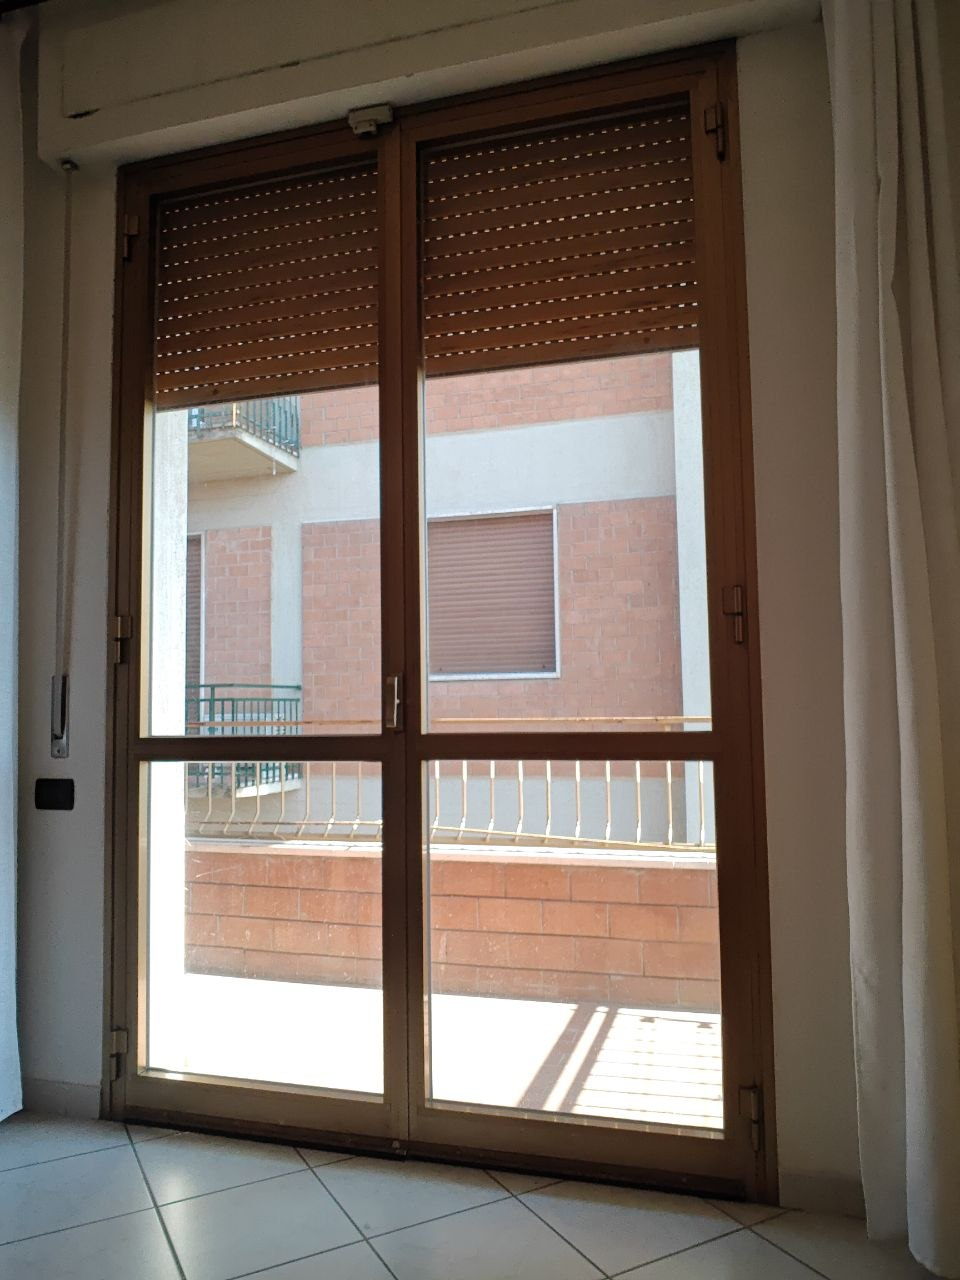
\includegraphics[width=\textwidth]{images/patchCore/p3_d2_fp_blind_ref.jpg}
    \caption{Reference (normal)}
    \label{fig:p3-d2-fp-blind-ref}
  \end{subfigure}
  \hfill
  \begin{subfigure}{0.42\textwidth}
    \centering
    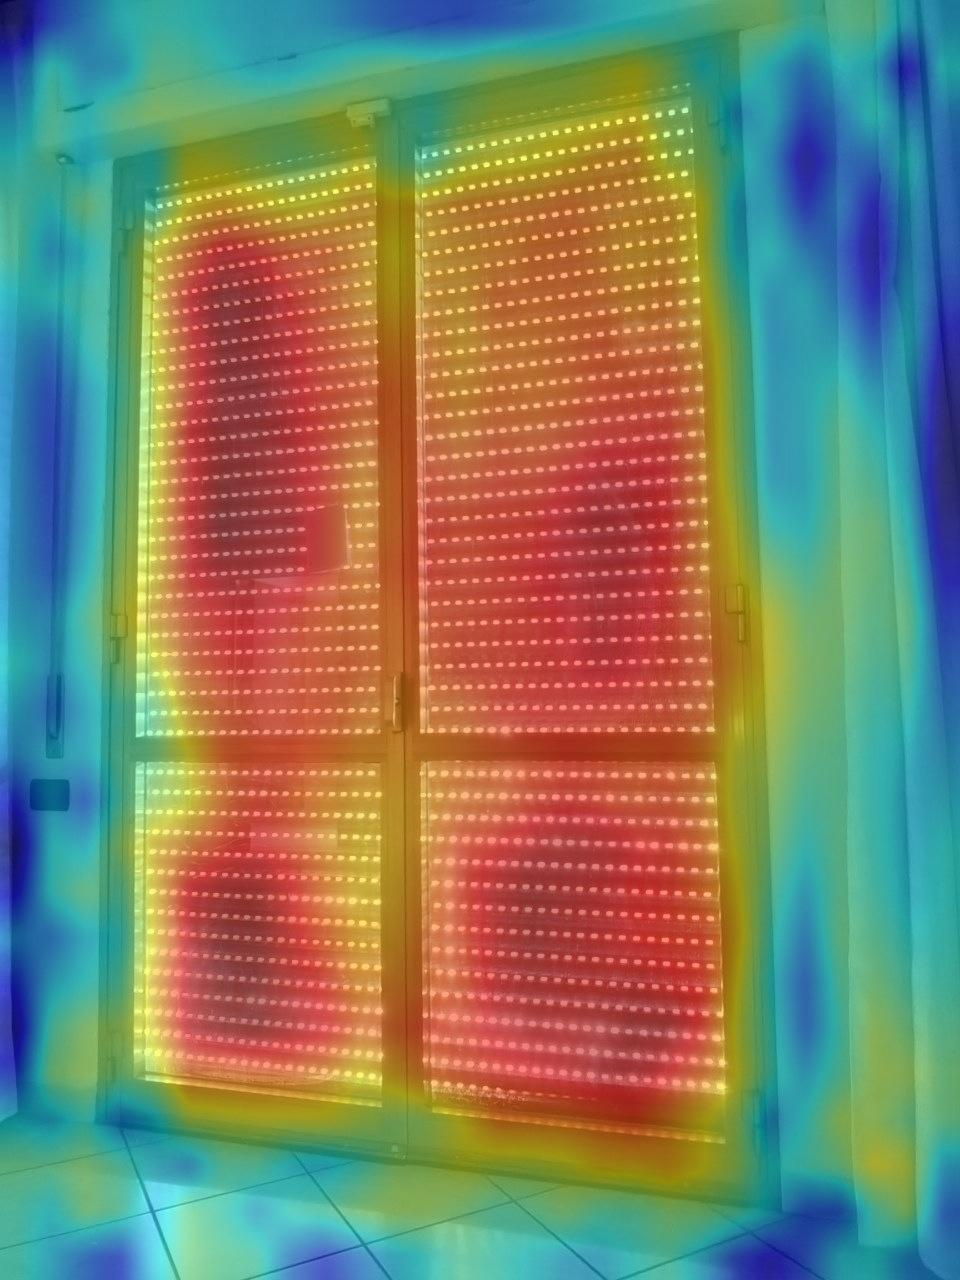
\includegraphics[width=\textwidth]{images/patchCore/p3_d2_fp_blind_heatmap.jpg}
    \caption{Anomaly heatmap}
    \label{fig:p3-d2-fp-blind-heatmap}
  \end{subfigure}
  \caption{Hard-negative false positive (worst case, score $3.873$) on a glass
  door. In the reference the external rolling shutter is up and the glass shows
  the courtyard outside; in the test frame the shutter is lowered, so the view
  through the panel changes completely. The background variation is too large for
  the fixed-camera assumption: the entire glazed area exceeds the anomaly
  threshold and overlaps the door frame, producing a false detection. This is a
  calibration limit of the static-background assumption, not a gating failure.}
  \label{fig:p3-d2-fp-blind}
\end{figure}

\subsubsection{Discussion}

Across the two phases, the failure modes of the method are diagnosable and
fixable within the PatchCore framework without architectural changes. Cast
shadows are addressed by disturbance-augmented, decoupled calibration that lifts
the per-camera threshold above the shadow band (shadow FPR $90.1\% \to 2.2\%$ at
SL-15); localised brightness excess is addressed symmetrically with light
variants; glass-door backgrounds are addressed by connected-component gating
exploiting the floor-grounding constraint; and threshold instability across
cameras is addressed by pooling the $\sigma$ estimate. The unifying finding is that none of these fixes
change the backbone's discriminative capacity, which is saturated; the bottleneck
is placing a single threshold robust to disturbances.

The conclusions carry two tiers of statistical weight. The synthetic calibration
phase (Phase~1, $N \approx 1000$) gives quantitative validations with adequate
power: the measured deltas of shadow augmentation, decoupling, and pooled
$\sigma$ are stable and generalisable to similar synthetic scenes. The real-world
phase (Phase~2, $N \approx$ tens) is a qualitative validation of the complete
pipeline: it confirms the expected
behaviour of gating plus pooled $\sigma$ and motivates the $k$ recalibration, but
the absolute numbers are illustrative, not a production benchmark. The structural
results - augmentation effectiveness, decoupling rationale, pooled-sigma variance
reduction, and the discrimination-versus-calibration mechanism - are pipeline
properties that generalise; the exact operating-point metrics should be
recalibrated for any new deployment using a site-specific $\sigma_{\mathrm{pop}}$
and a $k$ chosen from the application's cost ratio of false negatives to false
positives. Larger-scale quantitative validation of the gating on real glass
doors, conditioned on a semi-automatically annotated test set, is the natural
next step.

\subsection{Single-Class Obstruction Detection with YOLO (P1)}
\label{ssec:p1-results}

\subsubsection{Evaluation protocol}

The evaluation of P1 is organised in two macro-phases (Table~\ref{tab:p1-phases}),
mirroring the structure used for P3. \textbf{Phase~1} tests the
\emph{frozen-vocabulary hypothesis}: COCO-pretrained detectors used without any
fine-tuning, with a curated mapping of COCO classes onto the obstruction
concept. Its role is to establish, at zero training cost, the ceiling of the
``no fine-tuning'' route and to diagnose \emph{why} it falls short.
\textbf{Phase~2} fine-tunes the detectors of Table~\ref{tab:p1-models} on the
synthetic corpus and evaluates them at two levels: detection mAP on the
generative test set (D3) and image-level operational accuracy on the real
on-site set (D2), the latter shared with P3. Unless stated otherwise,
image-level decisions use the protocol of Chapter~\ref{chap:setup}
($\tau_{\mathrm{conf}} = 0.25$, minimum box area $1\%$).

\begin{table}[h]
  \centering
  \begin{tabular}{c l p{4.3cm} p{3.2cm}}
    \hline
    Phase & Data & Focus & Key metrics \\
    \hline
    1 & D1 + D2 & Frozen COCO detectors, class mapping, open-vocabulary variant & Image-level recall, F1, FPR \\
    2 & D3 + D2 & Fine-tuned detectors: localisation quality, real-world accuracy, capacity and architecture axes & mAP, instance/scene recall, F1 \\
    \hline
  \end{tabular}
  \caption{The two macro-phases of the P1 evaluation.}
  \label{tab:p1-phases}
\end{table}

\subsubsection{Phase 1: frozen-vocabulary baselines}

\paragraph{COCO class mapping.} A COCO-pretrained detector knows $80$ classes,
none of which is ``obstruction''. The baseline therefore counts a detection as
an obstruction when its class belongs to a hand-curated subset of COCO classes
semantically compatible with floor-standing obstacles (initially: bench,
backpack, handbag, suitcase, chair, couch, potted plant, bed, dining table,
refrigerator). With YOLO11n and this initial mapping, the result on the
synthetic corpus is a recall of $0.302$ at precision $0.929$ - the detector
misses about $70\%$ of the obstructions - and transfers to the real set at
recall $0.233$ with F1 $0.304$.

A per-class analysis on the $990$ positives and $110$ clean negatives
identifies both the false-positive drivers and the latent signal. The
\texttt{refrigerator} class fires on $11.8\%$ of the \emph{clean} negatives
(against $3.5\%$ of positives): visual inspection of all $49$ crops shows it
acting as a generic detector of large flat vertical panels - doors, not
refrigerators - and it is removed from the mapping. Conversely, objects with
wheels are systematically detected under vehicle classes: \texttt{bicycle}
fires on $9.9\%$ of positives and on \emph{zero} negatives, \texttt{motorcycle}
on $3.8\%$/$0\%$, because the detector recognises the wheels of carts and
wheelchairs; cylindrical waste bins fire on \texttt{toilet} ($47$ of $48$
detections on positives). The refined mapping (removing
\texttt{refrigerator} and \texttt{handbag}, adding \texttt{bicycle},
\texttt{motorcycle}, \texttt{toilet}, \texttt{vase}) improves the synthetic
metrics substantially (Table~\ref{tab:p1-mapping}).

\begin{table}[h]
  \centering
  \begin{tabular}{lcccc}
    \hline
    Mapping (YOLO11n, D1) & Recall & Precision & F1 & FPR \\
    \hline
    Initial ($10$ classes) & $0.302$ & $0.929$ & $0.456$ & $0.209$ \\
    Refined (final) & $0.406$ & $0.976$ & $\mathbf{0.574}$ & $0.091$ \\
    \hline
  \end{tabular}
  \caption{Phase 1: effect of the mapping refinement on the synthetic corpus.}
  \label{tab:p1-mapping}
\end{table}

The improvement, however, does \emph{not} transfer: on the real test set the
refined mapping produces a result identical to the previous one (recall
$0.200$, F1 $0.308$) - the \texttt{toilet} class, which detected the synthetic
cylindrical bins almost perfectly, fires on none of the real rectangular bins.
This is a concrete instance of the synthetic-to-real gap: a mapping adjustment
validated on clean synthetic crops is useless on real scenes, a warning that
recurs throughout this chapter.

\paragraph{Open-vocabulary variant.} YOLO-World \cite{Cheng2024yoloworld}
replaces the fixed vocabulary with text prompts, so the five obstacle
categories (plus synonyms) can be requested directly. On the synthetic corpus
it is nearly perfect (F1 $0.958$ at confidence $0.10$, FPR $0.064$); on the
real set it reaches recall $0.400$ and F1 $0.522$ - the best frozen result,
but still missing $60\%$ of real obstructions. The missed frames are almost
all of one kind: a free-standing floor fan blocking two of the six doors, an
object outside the prompt vocabulary. Adding explicit prompts for it
(\emph{ventilator, medical equipment, machine}) recovers almost nothing
($4$ weak detections out of $18$ frames), showing the object is intrinsically
hard for the open-vocabulary embedding, not merely un-prompted.

\paragraph{Frozen ceiling.} Table~\ref{tab:p1-frozen} collects all frozen
baselines on the real set. No frozen model exceeds F1 $0.52$; the differences
among them reflect mostly how liberally each fires generic COCO classes, not
their learning capacity. The conclusion of Phase~1 is structural: the
obstruction vocabulary of this domain (wheelchair, cart, stretcher, bin, box,
fan) is essentially absent from COCO, so no mapping or prompt engineering can
close the gap - the detector must be fine-tuned.

\begin{table}[h]
  \centering
  \begin{tabular}{llccccc}
    \hline
    Model & Type & Recall & Precision & F1 & FPR & Param.\ \\
    \hline
    YOLO-World-S & open-vocab.\ transformer & $0.400$ & $0.750$ & $\mathbf{0.520}$ & $0.111$ & $13.4$M \\
    Faster R-CNN MobileNet & CNN two-stage & $0.400$ & $0.545$ & $0.462$ & $0.278$ & $\sim$$19$M \\
    RT-DETR-L & transformer & $0.367$ & $0.440$ & $0.400$ & $0.389$ & $33$M \\
    Faster R-CNN ResNet50 & CNN two-stage & $0.267$ & $0.667$ & $0.381$ & $0.111$ & $\sim$$41$M \\
    YOLO11n & CNN one-stage & $0.200$ & $0.667$ & $0.308$ & $0.083$ & $2.6$M \\
    YOLO26n & CNN one-stage & $0.167$ & $1.000$ & $0.286$ & $0.000$ & $2.5$M \\
    \hline
  \end{tabular}
  \caption{Phase 1: all frozen baselines on the real test set (D2), image-level,
  $\tau_{\mathrm{conf}} = 0.25$, refined mapping (YOLO-World uses direct prompts
  instead). No frozen model reaches operational accuracy.}
  \label{tab:p1-frozen}
\end{table}

\subsubsection{Phase 2: fine-tuning}

\paragraph{Real-world accuracy (D2).} The fine-tuned YOLO11n, trained on the
full synthetic corpus, doubles the recall of its frozen counterpart on the real
set ($0.200 \to 0.400$) at F1 $0.490$ (Table~\ref{tab:p1-ft-poli}). The raw
recall, however, understates what the fine-tuning achieved, because the false
negatives are not uniformly distributed: of the $18$ missed obstructed frames,
$16$ contain the same free-standing floor fan already identified in Phase~1 -
an object belonging to \emph{none} of the five training categories, hence pure
out-of-distribution content - and only $2$ are genuine misses of an in-training
category (a waste bin, missed in two frames of one door). Restricted to the
frames whose obstacle belongs to a trained category, recall is $10/12 = 0.833$.
The fan is the same physical object that defeats P3's spatial gating
(Section~\ref{sec:p3-results}), but through an entirely different mechanism:
P3 detects it and loses it to a geometric rule, P1 simply has never seen one.
The comparison with Phase~1 is nonetheless sobering: the raw F1 of the
fine-tuned nano ($0.490$) does not clearly beat the best frozen baseline
(YOLO-World, $0.520$), and the advantage emerges only once the
out-of-vocabulary frames are accounted for - coverage of the object vocabulary,
not model quality, is the binding constraint on this test set.

\begin{table}[h]
  \centering
  \begin{tabular}{lcccccc}
    \hline
    YOLO11n on D2 & TP & FP & TN & FN & Recall & F1 \\
    \hline
    Frozen (refined mapping) & $6$ & $3$ & $33$ & $24$ & $0.200$ & $0.308$ \\
    Fine-tuned & $12$ & $7$ & $29$ & $18$ & $0.400$ & $0.490$ \\
    Fine-tuned, trained categories only & $10$ & -- & -- & $2$ & $0.833$ & -- \\
    \hline
  \end{tabular}
  \caption{Phase 2 on the real test set ($30$ obstructed, $36$ clear frames):
  fine-tuning versus the frozen baseline, and the recall restricted to frames
  whose obstacle belongs to a training category ($16$ of the $18$ false
  negatives contain the out-of-vocabulary floor fan).}
  \label{tab:p1-ft-poli}
\end{table}

\paragraph{Detection quality (D3).} On the generative test set the fine-tuned
YOLO11n reaches mAP$@50 = 0.866$ and mAP$@50$--$95 = 0.703$, with precision
$0.963$ and recall $0.831$ at the F1-optimal confidence. The gap between the
two mAP levels indicates that the residual weakness is localisation tightness
rather than object finding - a reading the next analysis makes precise. (An
earlier run of this evaluation forced $\tau_{\mathrm{conf}} = 0.25$ during mAP
computation and underestimated mAP$@50$ by about six points; all reported
values follow the correct protocol of Chapter~\ref{chap:setup}.)

\subsubsection{Instance-level versus scene-level reading}
\label{sssec:p1-metrics}

Qualitative inspection of the D3 errors shows a characteristic failure mode:
stacked cardboard boxes are detected as \emph{one} box spanning the pile
instead of $N$ separate instances. This section quantifies that observation
and, more importantly, examines what it does - and does not - imply for the
task. The analysis was run on the first release of D3 ($94$ images, $187$
instances, hand-assigned category tags).

Each ground-truth instance is classified by matching predictions at
$\mathrm{IoU} \geq 0.5$ (the mAP$@50$ rule) and, for the misses, by inspecting
the best-overlapping prediction: a miss is \emph{fused} when that prediction
overlaps the instance but was already claimed by a different ground-truth
object (one predicted box spanning several objects), \emph{loose} when a
prediction overlaps it without being matched to anything (imprecise
localisation), and \emph{isolated} when no prediction lies anywhere near.
Of $79$ misses, $16$ ($20\%$) are fused, $41$ ($52\%$) loose, and $22$
($28\%$) isolated - so nearly three quarters of the ``missed'' instances have
a prediction in their vicinity. The per-category breakdown is stark: the
\texttt{box} category has instance recall $0.281$ ($27/96$) against
$0.83$--$0.96$ for the other four categories, and \emph{all} fused misses
belong to it. The root cause is in the training data: the copy-paste generator
enforces a maximum pairwise IoU of $0.10$ between pasted objects
(Table~\ref{tab:ds-copypaste}), so the configuration ``several heavily
overlapping same-class objects'' is absent from training by construction, and
boxes are the only category the generative model habitually stacks.

Two observations prevent over-correcting for this. First, for heavily occluded
stacked objects the ground truth itself is ambiguous: whether three stacked
boxes ``are'' one object or three is an annotation convention (amodal versus
modal boxes), and either convention penalises one of the two plausible model
behaviours - the instance-level metric is partly ill-posed on such scenes,
independently of the model. Second, at the level that matters operationally -
is the route obstructed? - the failure disappears entirely: every scene of the
first release containing at least one box is flagged ($30/30$), a higher scene
rate than for scenes without boxes ($60/64$). The scene-level metric, however,
is biased in the opposite direction (a scene with five objects counts as
detected if one is found), so neither number alone is honest: the two bracket
the truth, and the clean signal in between is the \emph{isolated} miss count -
$22$ instances ($12$ of them boxes) that no prediction approaches, the only
misses that are genuine blind spots under any annotation convention. For a
single-class presence task, the stacked-box fusion is thus a metric artefact
rather than a functional defect, and no NMS or data intervention targeting it
was pursued.

\subsubsection{Background-leakage control}

As anticipated in Section~\ref{ssec:ds-gemini}, every D3 background also
appears in the training pool of the copy-paste corpus ($107$ stems as
composite backgrounds, $13$ as clean negatives): D3 could reward background
memorisation rather than object detection. The control is direct: YOLO11n was
retrained on the purged training set ($883$ positives, $97$ negatives) and
compared, on the identical D3 release, with the model trained on the full
corpus (Table~\ref{tab:p1-leak}).

\begin{table}[h]
  \centering
  \begin{tabular}{lcccc}
    \hline
    YOLO11n training set & mAP$@50$ & mAP$@50$--$95$ & Precision & Recall \\
    \hline
    Full corpus ($990/110$) & $0.863$ & $0.709$ & $0.951$ & $0.789$ \\
    Purged ($883/97$) & $0.866$ & $0.703$ & $0.963$ & $0.831$ \\
    \hline
  \end{tabular}
  \caption{Background-leakage control on D3: removing every training image that
  shares a background with the test set leaves the results unchanged.}
  \label{tab:p1-leak}
\end{table}

The two models are statistically indistinguishable - the purged model is even
marginally better. A complementary check on the first release found no recall
advantage on backgrounds seen as training positives over backgrounds seen only
as clean negatives ($0.588$ versus $0.545$). Background overlap therefore does
\emph{not} inflate the D3 numbers: the detector is reading the objects, not
recognising the scenes. All subsequent experiments nevertheless use the purged
training set, as the more defensible protocol.

\subsubsection{Capacity and architecture study}

With the protocol fixed, the remaining question is whether the choice of
detector matters: does more capacity, or a different architecture, buy real
generalisation? Seven models - three sizes per YOLO generation plus RT-DETR-L -
were trained identically on the purged corpus and evaluated on D3
(Table~\ref{tab:p1-scaling}).

\begin{table}[h]
  \centering
  \begin{tabular}{lcccccc}
    \hline
    Model & Param.\ & Synth.\ mAP$@50$--$95$ & \multicolumn{4}{c}{Generative test set (D3)} \\
     & & (internal val) & mAP$@50$ & mAP$@50$--$95$ & Prec.\ & Recall \\
    \hline
    YOLO11n & $2.6$M & $0.972$ & $\mathbf{0.866}$ & $0.703$ & $0.963$ & $0.831$ \\
    YOLO11s & $9.4$M & $0.986$ & $0.867$ & $0.709$ & $0.923$ & $0.837$ \\
    YOLO11m & $20.1$M & $0.984$ & $0.856$ & $0.708$ & $0.965$ & $0.837$ \\
    YOLO26n & $2.5$M & $0.982$ & $0.852$ & $0.708$ & $0.969$ & $0.789$ \\
    YOLO26s & $9.9$M & $0.978$ & $0.854$ & $0.698$ & $0.952$ & $0.840$ \\
    YOLO26m & $21.8$M & $0.982$ & $0.855$ & $\mathbf{0.716}$ & $0.952$ & $0.833$ \\
    RT-DETR-L & $32.8$M & $\mathbf{0.991}$ & $0.847$ & $0.702$ & $0.943$ & $0.801$ \\
    \hline
  \end{tabular}
  \caption{Capacity and architecture study, all models trained identically on
  the purged corpus. A $12.6\times$ parameter range moves D3 mAP$@50$ by two
  points with no monotone trend, while the internal synthetic validation is
  saturated for every model.}
  \label{tab:p1-scaling}
\end{table}

Three findings emerge. First, \emph{capacity buys nothing}: across a
$12.6\times$ parameter range, D3 mAP$@50$ spans $0.847$--$0.867$ with no
monotone trend - the spread is fold-to-fold noise, not signal. This echoes, in
a more extreme form, the small nano-to-XLarge gain ($+3.5$ mAP points)
reported by Miglionico et al.\ on real PPE data \cite{Miglionico2025}: on a
synthetic training corpus the capacity axis saturates entirely. Second,
\emph{the internal validation is saturated and non-predictive}: every model
scores $0.97$--$0.99$ on the held-out synthetic fold, and the ranking there
does not correlate with D3 - RT-DETR-L is the best model on synthetic data and
the worst on D3. Model selection on the synthetic validation would pick the
wrong model; only an external test set can rank these detectors. Third, the
bottleneck is the data, not the model: since no architecture or size moves the
external metric, the residual gap to perfect detection lies in the
synthetic-to-real distribution shift and in vocabulary coverage - consistent
with the fan analysis on D2.

\paragraph{RT-DETR training instability.} The RT-DETR result required one
protocol repair worth documenting. Trained with the default automatic mixed
precision, the run collapsed: validation losses turned \texttt{NaN}
sporadically from epoch $4$ and permanently from epoch $15$, at which point
every metric dropped to zero and early stopping ended the run at epoch $34$;
the usable checkpoint was the pre-collapse epoch $14$. This is a documented
failure mode of RT-DETR under AMP - fp16 overflow in the bipartite-matching
cost matrix \cite{UltralyticsRTDETRTrainer} - and the fix prescribed by the
framework documentation, disabling AMP with all else unchanged, resolved it
completely: the retrained run completed all $150$ epochs with zero \texttt{NaN}
and improved on D3 from mAP$@50$--$95 = 0.645$ to $0.702$ and recall from
$0.741$ to $0.801$. The single-variable repair attributes the instability to
AMP with certainty; Table~\ref{tab:p1-scaling} reports the repaired run. Even
so repaired, the transformer does not surpass the nano CNNs on D3 while
costing $12\times$ their memory - reinforcing, now on equal training footing,
that it is not the right candidate for this deployment.

\subsubsection{Discussion}

Across both phases, the failure modes of the detector pipeline are diagnosable
and consistent. Phase~1 establishes that the frozen-vocabulary route fails for
a structural reason - the domain's obstacle categories are absent from COCO -
and that the failure survives both mapping refinement and open-vocabulary
prompting; the per-class analysis (wheels detected as bicycles, bins as
toilets) shows the detectors \emph{see} the objects but cannot name them,
which is precisely the deficit fine-tuning repairs. Phase~2 shows that
fine-tuning on synthesis-derived labels transfers to real scenes for the
categories it covers (recall $0.833$ on trained categories) and fails
completely outside them (the floor fan, $16$ of $18$ false negatives): the
binding constraint is vocabulary coverage, not model choice, since a
$12.6\times$ capacity range and a CNN-to-transformer architecture change leave
the external metrics unmoved. The practical selection criterion then reduces
to cost, and the smallest model - YOLO11n, $5$~MB - is the rational deployment
candidate, a conclusion reached by measurement rather than by assumption.

The metric analysis of Section~\ref{sssec:p1-metrics} carries a lesson that
extends beyond P1: for a single-class presence task, instance-level detection
metrics and scene-level ones bracket the operational truth from opposite
sides, and on scenes with heavily occluded same-class objects the instance
ground truth is itself convention-dependent. Reporting a single headline
number would mislead in either direction; the defensible statement is the
decomposition - which misses are localisation artefacts and which are genuine
blind spots.

As for P3, the conclusions carry two tiers of statistical weight. The
synthetic and generative evaluations (D1, D3; hundreds of images) support the
structural findings - the vocabulary bottleneck, the capacity plateau, the
saturation of the internal validation. The real-set numbers (D2; tens of
frames) are a qualitative validation: they confirm the expected behaviour and
localise the failure modes, but the absolute values are illustrative. The
natural next step, enabled by the fold infrastructure already in place, is a
cross-validated estimate of the fold-to-fold variance of the D3 metrics, which
would put formal uncertainty bounds under the model comparison of
Table~\ref{tab:p1-scaling}.

\section{Application Results}

[Analysis of the end-to-end application results - to be completed.]
